\documentclass[twoside]{book}

% Packages required by doxygen
\usepackage{calc}
\usepackage{doxygen}
\usepackage{graphicx}
\usepackage[utf8]{inputenc}
\usepackage{makeidx}
\usepackage{multicol}
\usepackage{multirow}
\usepackage{textcomp}
\usepackage[table]{xcolor}

% Font selection
\usepackage[T1]{fontenc}
\usepackage{mathptmx}
\usepackage[scaled=.90]{helvet}
\usepackage{courier}
\usepackage{amssymb}
\usepackage{sectsty}
\renewcommand{\familydefault}{\sfdefault}
\allsectionsfont{%
  \fontseries{bc}\selectfont%
  \color{darkgray}%
}
\renewcommand{\DoxyLabelFont}{%
  \fontseries{bc}\selectfont%
  \color{darkgray}%
}

% Page & text layout
\usepackage{geometry}
\geometry{%
  a4paper,%
  top=2.5cm,%
  bottom=2.5cm,%
  left=2.5cm,%
  right=2.5cm%
}
\tolerance=750
\hfuzz=15pt
\hbadness=750
\setlength{\emergencystretch}{15pt}
\setlength{\parindent}{0cm}
\setlength{\parskip}{0.2cm}
\makeatletter
\renewcommand{\paragraph}{%
  \@startsection{paragraph}{4}{0ex}{-1.0ex}{1.0ex}{%
    \normalfont\normalsize\bfseries\SS@parafont%
  }%
}
\renewcommand{\subparagraph}{%
  \@startsection{subparagraph}{5}{0ex}{-1.0ex}{1.0ex}{%
    \normalfont\normalsize\bfseries\SS@subparafont%
  }%
}
\makeatother

% Headers & footers
\usepackage{fancyhdr}
\pagestyle{fancyplain}
\fancyhead[LE]{\fancyplain{}{\bfseries\thepage}}
\fancyhead[CE]{\fancyplain{}{}}
\fancyhead[RE]{\fancyplain{}{\bfseries\leftmark}}
\fancyhead[LO]{\fancyplain{}{\bfseries\rightmark}}
\fancyhead[CO]{\fancyplain{}{}}
\fancyhead[RO]{\fancyplain{}{\bfseries\thepage}}
\fancyfoot[LE]{\fancyplain{}{}}
\fancyfoot[CE]{\fancyplain{}{}}
\fancyfoot[RE]{\fancyplain{}{\bfseries\scriptsize Generated on Thu May 18 2017 20\-:03\-:52 for L\-D\-A\-P P\-W Changer by Doxygen }}
\fancyfoot[LO]{\fancyplain{}{\bfseries\scriptsize Generated on Thu May 18 2017 20\-:03\-:52 for L\-D\-A\-P P\-W Changer by Doxygen }}
\fancyfoot[CO]{\fancyplain{}{}}
\fancyfoot[RO]{\fancyplain{}{}}
\renewcommand{\footrulewidth}{0.4pt}
\renewcommand{\chaptermark}[1]{%
  \markboth{#1}{}%
}
\renewcommand{\sectionmark}[1]{%
  \markright{\thesection\ #1}%
}

% Indices & bibliography
\usepackage{natbib}
\usepackage[titles]{tocloft}
\setcounter{tocdepth}{3}
\setcounter{secnumdepth}{5}
\makeindex

% Hyperlinks (required, but should be loaded last)
\usepackage{ifpdf}
\ifpdf
  \usepackage[pdftex,pagebackref=true]{hyperref}
\else
  \usepackage[ps2pdf,pagebackref=true]{hyperref}
\fi
\hypersetup{%
  colorlinks=true,%
  linkcolor=blue,%
  citecolor=blue,%
  unicode%
}

% Custom commands
\newcommand{\clearemptydoublepage}{%
  \newpage{\pagestyle{empty}\cleardoublepage}%
}


%===== C O N T E N T S =====

\begin{document}

% Titlepage & ToC
\hypersetup{pageanchor=false}
\pagenumbering{roman}
\begin{titlepage}
\vspace*{7cm}
\begin{center}%
{\Large L\-D\-A\-P P\-W Changer }\\
\vspace*{1cm}
{\large Generated by Doxygen 1.8.5}\\
\vspace*{0.5cm}
{\small Thu May 18 2017 20:03:52}\\
\end{center}
\end{titlepage}
\clearemptydoublepage
\tableofcontents
\clearemptydoublepage
\pagenumbering{arabic}
\hypersetup{pageanchor=true}

%--- Begin generated contents ---
\chapter{wsgi script to change a users ldap password}
\label{md__home_war_git_bmb_ldap_pwchange_package_pk_README}
\hypertarget{md__home_war_git_bmb_ldap_pwchange_package_pk_README}{}
with authentication already done 
\chapter{wsgi script to change a users ldap password}
\label{md__home_war_git_bmb_ldap_pwchange_README}
\hypertarget{md__home_war_git_bmb_ldap_pwchange_README}{}
with authentication already done 
\chapter{Hierarchical Index}
\section{Class Hierarchy}
This inheritance list is sorted roughly, but not completely, alphabetically\-:\begin{DoxyCompactList}
\item Exception\begin{DoxyCompactList}
\item \contentsline{section}{ldap.\-ldap.\-L\-D\-A\-P\-User\-Search\-Found\-No\-User\-Exception}{\pageref{classldap_1_1ldap_1_1LDAPUserSearchFoundNoUserException}}{}
\item \contentsline{section}{ldap.\-ldap.\-L\-D\-A\-P\-User\-Search\-Found\-No\-User\-Exception}{\pageref{classldap_1_1ldap_1_1LDAPUserSearchFoundNoUserException}}{}
\item \contentsline{section}{ldap.\-ldap.\-L\-D\-A\-P\-User\-Search\-Found\-Too\-Many\-Users\-Exception}{\pageref{classldap_1_1ldap_1_1LDAPUserSearchFoundTooManyUsersException}}{}
\item \contentsline{section}{ldap.\-ldap.\-L\-D\-A\-P\-User\-Search\-Found\-Too\-Many\-Users\-Exception}{\pageref{classldap_1_1ldap_1_1LDAPUserSearchFoundTooManyUsersException}}{}
\item \contentsline{section}{password.\-password.\-Password\-Too\-Short\-Exception}{\pageref{classpassword_1_1password_1_1PasswordTooShortException}}{}
\item \contentsline{section}{password.\-password.\-Password\-Too\-Short\-Exception}{\pageref{classpassword_1_1password_1_1PasswordTooShortException}}{}
\end{DoxyCompactList}
\item object\begin{DoxyCompactList}
\item \contentsline{section}{ldap.\-ldap.\-L\-D\-A\-P\-Configuration}{\pageref{classldap_1_1ldap_1_1LDAPConfiguration}}{}
\item \contentsline{section}{ldap.\-ldap.\-L\-D\-A\-P\-Configuration}{\pageref{classldap_1_1ldap_1_1LDAPConfiguration}}{}
\item \contentsline{section}{ldap.\-ldap.\-L\-D\-A\-P\-Connection}{\pageref{classldap_1_1ldap_1_1LDAPConnection}}{}
\item \contentsline{section}{ldap.\-ldap.\-L\-D\-A\-P\-Connection}{\pageref{classldap_1_1ldap_1_1LDAPConnection}}{}
\item \contentsline{section}{ldap.\-ldap.\-L\-D\-A\-P\-Filter}{\pageref{classldap_1_1ldap_1_1LDAPFilter}}{}
\item \contentsline{section}{ldap.\-ldap.\-L\-D\-A\-P\-Filter}{\pageref{classldap_1_1ldap_1_1LDAPFilter}}{}
\item \contentsline{section}{ldap.\-ldap.\-L\-D\-A\-P\-Filter\-Item}{\pageref{classldap_1_1ldap_1_1LDAPFilterItem}}{}
\item \contentsline{section}{ldap.\-ldap.\-L\-D\-A\-P\-Filter\-Item}{\pageref{classldap_1_1ldap_1_1LDAPFilterItem}}{}
\item \contentsline{section}{password.\-password.\-Escaped\-Part}{\pageref{classpassword_1_1password_1_1EscapedPart}}{}
\item \contentsline{section}{password.\-password.\-Escaped\-Part}{\pageref{classpassword_1_1password_1_1EscapedPart}}{}
\item \contentsline{section}{password.\-password.\-Password}{\pageref{classpassword_1_1password_1_1Password}}{}
\item \contentsline{section}{password.\-password.\-Password}{\pageref{classpassword_1_1password_1_1Password}}{}
\item \contentsline{section}{session.\-Session\-Store}{\pageref{classsession_1_1SessionStore}}{}
\item \contentsline{section}{session.\-Session\-Store}{\pageref{classsession_1_1SessionStore}}{}
\item \contentsline{section}{tools.\-tools.\-Log}{\pageref{classtools_1_1tools_1_1Log}}{}
\item \contentsline{section}{tools.\-tools.\-Log}{\pageref{classtools_1_1tools_1_1Log}}{}
\item \contentsline{section}{wzserver.\-Wz\-Server}{\pageref{classwzserver_1_1WzServer}}{}
\begin{DoxyCompactList}
\item \contentsline{section}{service.\-Pw\-Change\-Server}{\pageref{classservice_1_1PwChangeServer}}{}
\item \contentsline{section}{service.\-Pw\-Change\-Server}{\pageref{classservice_1_1PwChangeServer}}{}
\end{DoxyCompactList}
\item \contentsline{section}{wzserver.\-Wz\-Server}{\pageref{classwzserver_1_1WzServer}}{}
\end{DoxyCompactList}
\item L\-D\-A\-P\-Configuration\begin{DoxyCompactList}
\item \contentsline{section}{config.\-Config}{\pageref{classconfig_1_1Config}}{}
\item \contentsline{section}{config.\-Config}{\pageref{classconfig_1_1Config}}{}
\end{DoxyCompactList}
\end{DoxyCompactList}

\chapter{Class Index}
\section{Class List}
Here are the classes, structs, unions and interfaces with brief descriptions\-:\begin{DoxyCompactList}
\item\contentsline{section}{\hyperlink{classconfig_1_1Config}{config.\-Config} }{\pageref{classconfig_1_1Config}}{}
\item\contentsline{section}{\hyperlink{classpassword_1_1password_1_1EscapedPart}{password.\-password.\-Escaped\-Part} }{\pageref{classpassword_1_1password_1_1EscapedPart}}{}
\item\contentsline{section}{\hyperlink{classldap_1_1ldap_1_1LDAPConfiguration}{ldap.\-ldap.\-L\-D\-A\-P\-Configuration} }{\pageref{classldap_1_1ldap_1_1LDAPConfiguration}}{}
\item\contentsline{section}{\hyperlink{classldap_1_1ldap_1_1LDAPConnection}{ldap.\-ldap.\-L\-D\-A\-P\-Connection} }{\pageref{classldap_1_1ldap_1_1LDAPConnection}}{}
\item\contentsline{section}{\hyperlink{classldap_1_1ldap_1_1LDAPFilter}{ldap.\-ldap.\-L\-D\-A\-P\-Filter} }{\pageref{classldap_1_1ldap_1_1LDAPFilter}}{}
\item\contentsline{section}{\hyperlink{classldap_1_1ldap_1_1LDAPFilterItem}{ldap.\-ldap.\-L\-D\-A\-P\-Filter\-Item} }{\pageref{classldap_1_1ldap_1_1LDAPFilterItem}}{}
\item\contentsline{section}{\hyperlink{classldap_1_1ldap_1_1LDAPUserSearchFoundNoUserException}{ldap.\-ldap.\-L\-D\-A\-P\-User\-Search\-Found\-No\-User\-Exception} }{\pageref{classldap_1_1ldap_1_1LDAPUserSearchFoundNoUserException}}{}
\item\contentsline{section}{\hyperlink{classldap_1_1ldap_1_1LDAPUserSearchFoundTooManyUsersException}{ldap.\-ldap.\-L\-D\-A\-P\-User\-Search\-Found\-Too\-Many\-Users\-Exception} }{\pageref{classldap_1_1ldap_1_1LDAPUserSearchFoundTooManyUsersException}}{}
\item\contentsline{section}{\hyperlink{classtools_1_1tools_1_1Log}{tools.\-tools.\-Log} }{\pageref{classtools_1_1tools_1_1Log}}{}
\item\contentsline{section}{\hyperlink{classpassword_1_1password_1_1Password}{password.\-password.\-Password} }{\pageref{classpassword_1_1password_1_1Password}}{}
\item\contentsline{section}{\hyperlink{classpassword_1_1password_1_1PasswordTooShortException}{password.\-password.\-Password\-Too\-Short\-Exception} }{\pageref{classpassword_1_1password_1_1PasswordTooShortException}}{}
\item\contentsline{section}{\hyperlink{classservice_1_1PwChangeServer}{service.\-Pw\-Change\-Server} }{\pageref{classservice_1_1PwChangeServer}}{}
\item\contentsline{section}{\hyperlink{classsession_1_1SessionStore}{session.\-Session\-Store} }{\pageref{classsession_1_1SessionStore}}{}
\item\contentsline{section}{\hyperlink{classwzserver_1_1WzServer}{wzserver.\-Wz\-Server} }{\pageref{classwzserver_1_1WzServer}}{}
\end{DoxyCompactList}

\chapter{Class Documentation}
\hypertarget{classconfig_1_1Config}{\section{config.\-Config Class Reference}
\label{classconfig_1_1Config}\index{config.\-Config@{config.\-Config}}
}
Inheritance diagram for config.\-Config\-:\begin{figure}[H]
\begin{center}
\leavevmode
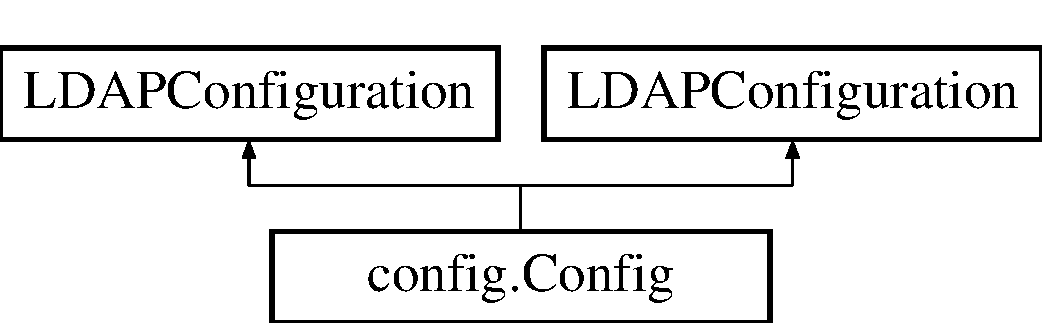
\includegraphics[height=2.000000cm]{classconfig_1_1Config}
\end{center}
\end{figure}
\subsection*{Public Member Functions}
\begin{DoxyCompactItemize}
\item 
\hypertarget{classconfig_1_1Config_a2c77f4b64c0bf70b283cdb4af4c93fa1}{def {\bfseries \-\_\-\-\_\-init\-\_\-\-\_\-}}\label{classconfig_1_1Config_a2c77f4b64c0bf70b283cdb4af4c93fa1}

\item 
\hypertarget{classconfig_1_1Config_a2c77f4b64c0bf70b283cdb4af4c93fa1}{def {\bfseries \-\_\-\-\_\-init\-\_\-\-\_\-}}\label{classconfig_1_1Config_a2c77f4b64c0bf70b283cdb4af4c93fa1}

\end{DoxyCompactItemize}
\subsection*{Static Public Attributes}
\begin{DoxyCompactItemize}
\item 
\hypertarget{classconfig_1_1Config_a274d1112585561b071ba84299e30142a}{list {\bfseries L\-D\-A\-P\-\_\-\-R\-O\-O\-T\-\_\-\-P\-A\-S\-S\-W\-O\-R\-D} = os.\-environ\mbox{[}'R\-O\-O\-T\-P\-W'\mbox{]}}\label{classconfig_1_1Config_a274d1112585561b071ba84299e30142a}

\item 
\hypertarget{classconfig_1_1Config_a484d232d78b4f414d8066799a237d451}{list {\bfseries S\-L\-A\-P\-D\-P\-O\-R\-T} = os.\-environ\mbox{[}'S\-L\-A\-P\-D\-P\-O\-R\-T'\mbox{]}}\label{classconfig_1_1Config_a484d232d78b4f414d8066799a237d451}

\item 
\hypertarget{classconfig_1_1Config_ab2fdceff538b5908c1d4f88eadab3c5b}{list {\bfseries S\-L\-A\-P\-D\-H\-O\-S\-T} = os.\-environ\mbox{[}'S\-L\-A\-P\-D\-H\-O\-S\-T'\mbox{]}}\label{classconfig_1_1Config_ab2fdceff538b5908c1d4f88eadab3c5b}

\item 
\hypertarget{classconfig_1_1Config_aedc19cf03da3edc6b41841a6c00491a8}{list {\bfseries R\-O\-O\-T\-D\-N} = os.\-environ\mbox{[}'R\-O\-O\-T\-D\-N'\mbox{]}}\label{classconfig_1_1Config_aedc19cf03da3edc6b41841a6c00491a8}

\item 
\hypertarget{classconfig_1_1Config_a8c5c6504477e14ea7c9086a165c17150}{list {\bfseries A\-D\-M\-I\-N\-D\-N} = os.\-environ\mbox{[}'A\-D\-M\-I\-N\-D\-N'\mbox{]}}\label{classconfig_1_1Config_a8c5c6504477e14ea7c9086a165c17150}

\item 
\hypertarget{classconfig_1_1Config_ac85c1a894f69b1fd6a5e8997e0066ff9}{list {\bfseries U\-S\-E\-R\-N\-A\-M\-E\-\_\-\-I\-N} = os.\-environ\mbox{[}'U\-S\-E\-R\-N\-A\-M\-E\-\_\-\-I\-N'\mbox{]}}\label{classconfig_1_1Config_ac85c1a894f69b1fd6a5e8997e0066ff9}

\item 
\hypertarget{classconfig_1_1Config_a9b2b96d80a364b00eb74f09cbc300dc4}{list {\bfseries U\-S\-E\-R\-\_\-\-T\-O\-\_\-\-D\-N} = os.\-environ\mbox{[}'U\-S\-E\-R\-\_\-\-T\-O\-\_\-\-D\-N'\mbox{]}}\label{classconfig_1_1Config_a9b2b96d80a364b00eb74f09cbc300dc4}

\end{DoxyCompactItemize}


\subsection{Detailed Description}
\begin{DoxyVerb}Configuration object.

    Configuration is loaded from the process environment.
    
    Look into LDAPConfiguration for parameters.\end{DoxyVerb}
 

The documentation for this class was generated from the following files\-:\begin{DoxyCompactItemize}
\item 
/home/war/git/bmb/ldap\-\_\-pwchange/config.\-py\item 
/home/war/git/bmb/ldap\-\_\-pwchange/package/pk/config.\-py\end{DoxyCompactItemize}

\hypertarget{classpassword_1_1password_1_1EscapedPart}{\section{password.\-password.\-Escaped\-Part Class Reference}
\label{classpassword_1_1password_1_1EscapedPart}\index{password.\-password.\-Escaped\-Part@{password.\-password.\-Escaped\-Part}}
}
Inheritance diagram for password.\-password.\-Escaped\-Part\-:\begin{figure}[H]
\begin{center}
\leavevmode
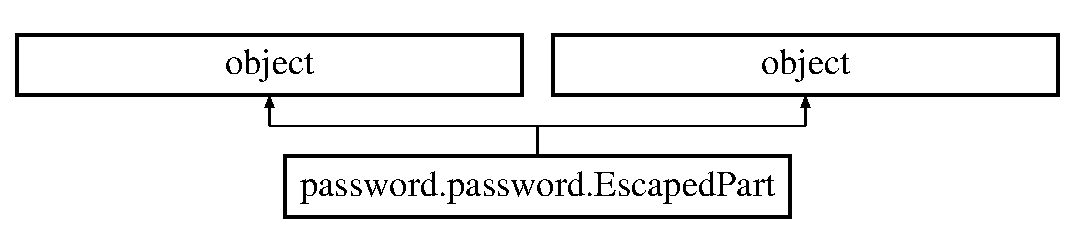
\includegraphics[height=2.000000cm]{classpassword_1_1password_1_1EscapedPart}
\end{center}
\end{figure}
\subsection*{Public Member Functions}
\begin{DoxyCompactItemize}
\item 
\hypertarget{classpassword_1_1password_1_1EscapedPart_ac0480fa8b823e218d2a159c00b2af28e}{def {\bfseries \-\_\-\-\_\-init\-\_\-\-\_\-}}\label{classpassword_1_1password_1_1EscapedPart_ac0480fa8b823e218d2a159c00b2af28e}

\item 
\hypertarget{classpassword_1_1password_1_1EscapedPart_aa6c689420d06baffb374a01035dad908}{def {\bfseries \-\_\-\-\_\-str\-\_\-\-\_\-}}\label{classpassword_1_1password_1_1EscapedPart_aa6c689420d06baffb374a01035dad908}

\item 
\hypertarget{classpassword_1_1password_1_1EscapedPart_ac0480fa8b823e218d2a159c00b2af28e}{def {\bfseries \-\_\-\-\_\-init\-\_\-\-\_\-}}\label{classpassword_1_1password_1_1EscapedPart_ac0480fa8b823e218d2a159c00b2af28e}

\item 
\hypertarget{classpassword_1_1password_1_1EscapedPart_aa6c689420d06baffb374a01035dad908}{def {\bfseries \-\_\-\-\_\-str\-\_\-\-\_\-}}\label{classpassword_1_1password_1_1EscapedPart_aa6c689420d06baffb374a01035dad908}

\end{DoxyCompactItemize}
\subsection*{Public Attributes}
\begin{DoxyCompactItemize}
\item 
\hypertarget{classpassword_1_1password_1_1EscapedPart_af85d9281da5f007ce53ebb24cef34e55}{{\bfseries txt}}\label{classpassword_1_1password_1_1EscapedPart_af85d9281da5f007ce53ebb24cef34e55}

\item 
\hypertarget{classpassword_1_1password_1_1EscapedPart_a68a915571f1632854c640ff08a0c03ca}{{\bfseries escaped}}\label{classpassword_1_1password_1_1EscapedPart_a68a915571f1632854c640ff08a0c03ca}

\end{DoxyCompactItemize}


The documentation for this class was generated from the following files\-:\begin{DoxyCompactItemize}
\item 
/home/war/git/bmb/ldap\-\_\-pwchange/package/pk/password/password.\-py\item 
/home/war/git/bmb/ldap\-\_\-pwchange/password/password.\-py\end{DoxyCompactItemize}

\hypertarget{classldap_1_1ldap_1_1LDAPConfiguration}{\section{ldap.\-ldap.\-L\-D\-A\-P\-Configuration Class Reference}
\label{classldap_1_1ldap_1_1LDAPConfiguration}\index{ldap.\-ldap.\-L\-D\-A\-P\-Configuration@{ldap.\-ldap.\-L\-D\-A\-P\-Configuration}}
}
Inheritance diagram for ldap.\-ldap.\-L\-D\-A\-P\-Configuration\-:\begin{figure}[H]
\begin{center}
\leavevmode
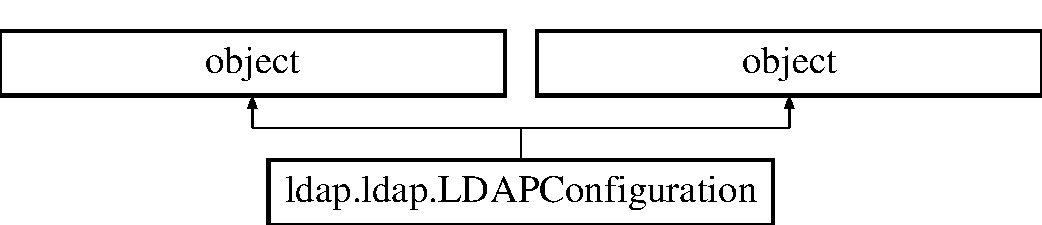
\includegraphics[height=2.000000cm]{classldap_1_1ldap_1_1LDAPConfiguration}
\end{center}
\end{figure}
\subsection*{Public Member Functions}
\begin{DoxyCompactItemize}
\item 
\hypertarget{classldap_1_1ldap_1_1LDAPConfiguration_a8402c008a22021c6d8c300fbb84515b4}{def {\bfseries \-\_\-\-\_\-init\-\_\-\-\_\-}}\label{classldap_1_1ldap_1_1LDAPConfiguration_a8402c008a22021c6d8c300fbb84515b4}

\item 
\hypertarget{classldap_1_1ldap_1_1LDAPConfiguration_a8402c008a22021c6d8c300fbb84515b4}{def {\bfseries \-\_\-\-\_\-init\-\_\-\-\_\-}}\label{classldap_1_1ldap_1_1LDAPConfiguration_a8402c008a22021c6d8c300fbb84515b4}

\end{DoxyCompactItemize}
\subsection*{Public Attributes}
\begin{DoxyCompactItemize}
\item 
\hypertarget{classldap_1_1ldap_1_1LDAPConfiguration_aaf42a56c4cc906ef054c6330e792edfb}{{\bfseries S\-L\-A\-P\-D\-H\-O\-S\-T}}\label{classldap_1_1ldap_1_1LDAPConfiguration_aaf42a56c4cc906ef054c6330e792edfb}

\item 
\hypertarget{classldap_1_1ldap_1_1LDAPConfiguration_ad2f5d28dbacb48734bc80310057f7125}{{\bfseries server}}\label{classldap_1_1ldap_1_1LDAPConfiguration_ad2f5d28dbacb48734bc80310057f7125}

\end{DoxyCompactItemize}
\subsection*{Static Public Attributes}
\begin{DoxyCompactItemize}
\item 
\hypertarget{classldap_1_1ldap_1_1LDAPConfiguration_a1b68249f32a9990f6f4fb75ff20f88ba}{list {\bfseries L\-D\-A\-P\-\_\-\-R\-O\-O\-T\-\_\-\-P\-A\-S\-S\-W\-O\-R\-D} = os.\-environ\mbox{[}'R\-O\-O\-T\-P\-W'\mbox{]}}\label{classldap_1_1ldap_1_1LDAPConfiguration_a1b68249f32a9990f6f4fb75ff20f88ba}

\item 
\hypertarget{classldap_1_1ldap_1_1LDAPConfiguration_a187f1bd89a4bbc7d7cbb9aa9f0431f2f}{list {\bfseries S\-L\-A\-P\-D\-P\-O\-R\-T} = os.\-environ\mbox{[}'S\-L\-A\-P\-D\-P\-O\-R\-T'\mbox{]}}\label{classldap_1_1ldap_1_1LDAPConfiguration_a187f1bd89a4bbc7d7cbb9aa9f0431f2f}

\item 
\hypertarget{classldap_1_1ldap_1_1LDAPConfiguration_a6f7c3a9f138dc9697ca5494d322808a3}{list {\bfseries S\-L\-A\-P\-D\-H\-O\-S\-T} = os.\-environ\mbox{[}'S\-L\-A\-P\-D\-H\-O\-S\-T'\mbox{]}}\label{classldap_1_1ldap_1_1LDAPConfiguration_a6f7c3a9f138dc9697ca5494d322808a3}

\item 
\hypertarget{classldap_1_1ldap_1_1LDAPConfiguration_a73e91ac4ac6d5d2ae4f30dc97d70e433}{list {\bfseries R\-O\-O\-T\-D\-N} = os.\-environ\mbox{[}'R\-O\-O\-T\-D\-N'\mbox{]}}\label{classldap_1_1ldap_1_1LDAPConfiguration_a73e91ac4ac6d5d2ae4f30dc97d70e433}

\item 
\hypertarget{classldap_1_1ldap_1_1LDAPConfiguration_a5d2425ffe420acb07721f6bbc8514656}{list {\bfseries A\-D\-M\-I\-N\-D\-N} = os.\-environ\mbox{[}'A\-D\-M\-I\-N\-D\-N'\mbox{]}}\label{classldap_1_1ldap_1_1LDAPConfiguration_a5d2425ffe420acb07721f6bbc8514656}

\item 
\hypertarget{classldap_1_1ldap_1_1LDAPConfiguration_ae7bfc302e4a58797cfcd52d91c73d197}{list {\bfseries U\-S\-E\-R\-N\-A\-M\-E\-\_\-\-I\-N} = os.\-environ\mbox{[}'U\-S\-E\-R\-N\-A\-M\-E\-\_\-\-I\-N'\mbox{]}}\label{classldap_1_1ldap_1_1LDAPConfiguration_ae7bfc302e4a58797cfcd52d91c73d197}

\item 
\hypertarget{classldap_1_1ldap_1_1LDAPConfiguration_aa4631e2781b16bd84dba30eff70acb24}{list {\bfseries U\-S\-E\-R\-\_\-\-T\-O\-\_\-\-D\-N} = os.\-environ\mbox{[}'U\-S\-E\-R\-\_\-\-T\-O\-\_\-\-D\-N'\mbox{]}}\label{classldap_1_1ldap_1_1LDAPConfiguration_aa4631e2781b16bd84dba30eff70acb24}

\end{DoxyCompactItemize}


\subsection{Detailed Description}
\begin{DoxyVerb}Configuration object.

     Loads the config from the process environment.

     Users should know what to put into most of these, except:

     USERNAME_IN :
         The apache (request) environment variable where the username (dn) is found.
     USER_TO_DN: 
         Simple way to expand the username into a dn. Like "uid={}, dc=example, dc=com"\end{DoxyVerb}
 

The documentation for this class was generated from the following files\-:\begin{DoxyCompactItemize}
\item 
/home/war/git/bmb/ldap\-\_\-pwchange/ldap/ldap.\-py\item 
/home/war/git/bmb/ldap\-\_\-pwchange/package/pk/ldap/ldap.\-py\end{DoxyCompactItemize}

\hypertarget{classldap_1_1ldap_1_1LDAPConnection}{\section{ldap.\-ldap.\-L\-D\-A\-P\-Connection Class Reference}
\label{classldap_1_1ldap_1_1LDAPConnection}\index{ldap.\-ldap.\-L\-D\-A\-P\-Connection@{ldap.\-ldap.\-L\-D\-A\-P\-Connection}}
}
Inheritance diagram for ldap.\-ldap.\-L\-D\-A\-P\-Connection\-:\begin{figure}[H]
\begin{center}
\leavevmode
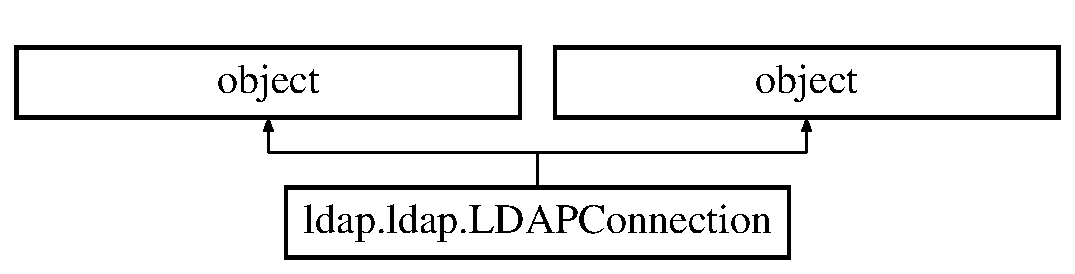
\includegraphics[height=2.000000cm]{classldap_1_1ldap_1_1LDAPConnection}
\end{center}
\end{figure}
\subsection*{Public Member Functions}
\begin{DoxyCompactItemize}
\item 
def \hyperlink{classldap_1_1ldap_1_1LDAPConnection_a7f55602eaeb5d3e6d6076850ef1effbd}{\-\_\-\-\_\-init\-\_\-\-\_\-}
\item 
\hypertarget{classldap_1_1ldap_1_1LDAPConnection_a8a21a52d52537ec1b508768214698540}{def {\bfseries search\-\_\-user}}\label{classldap_1_1ldap_1_1LDAPConnection_a8a21a52d52537ec1b508768214698540}

\item 
\hypertarget{classldap_1_1ldap_1_1LDAPConnection_ab11fe1e8f34ce63cb12b78aa75aec55d}{def {\bfseries search}}\label{classldap_1_1ldap_1_1LDAPConnection_ab11fe1e8f34ce63cb12b78aa75aec55d}

\item 
\hypertarget{classldap_1_1ldap_1_1LDAPConnection_a1c7661061babcba2c8625fc929cc99cc}{def {\bfseries change\-\_\-password}}\label{classldap_1_1ldap_1_1LDAPConnection_a1c7661061babcba2c8625fc929cc99cc}

\item 
\hypertarget{classldap_1_1ldap_1_1LDAPConnection_a8b034f2c41f799d27c8e7982a2af5f5b}{def {\bfseries dump\-\_\-testuser}}\label{classldap_1_1ldap_1_1LDAPConnection_a8b034f2c41f799d27c8e7982a2af5f5b}

\item 
\hypertarget{classldap_1_1ldap_1_1LDAPConnection_aaa167752ae9dff812be4b2598fae1d5b}{def {\bfseries test\-\_\-userdn\-\_\-password}}\label{classldap_1_1ldap_1_1LDAPConnection_aaa167752ae9dff812be4b2598fae1d5b}

\item 
def \hyperlink{classldap_1_1ldap_1_1LDAPConnection_a7f55602eaeb5d3e6d6076850ef1effbd}{\-\_\-\-\_\-init\-\_\-\-\_\-}
\item 
\hypertarget{classldap_1_1ldap_1_1LDAPConnection_a8a21a52d52537ec1b508768214698540}{def {\bfseries search\-\_\-user}}\label{classldap_1_1ldap_1_1LDAPConnection_a8a21a52d52537ec1b508768214698540}

\item 
\hypertarget{classldap_1_1ldap_1_1LDAPConnection_ab11fe1e8f34ce63cb12b78aa75aec55d}{def {\bfseries search}}\label{classldap_1_1ldap_1_1LDAPConnection_ab11fe1e8f34ce63cb12b78aa75aec55d}

\item 
\hypertarget{classldap_1_1ldap_1_1LDAPConnection_a1c7661061babcba2c8625fc929cc99cc}{def {\bfseries change\-\_\-password}}\label{classldap_1_1ldap_1_1LDAPConnection_a1c7661061babcba2c8625fc929cc99cc}

\item 
\hypertarget{classldap_1_1ldap_1_1LDAPConnection_a8b034f2c41f799d27c8e7982a2af5f5b}{def {\bfseries dump\-\_\-testuser}}\label{classldap_1_1ldap_1_1LDAPConnection_a8b034f2c41f799d27c8e7982a2af5f5b}

\item 
\hypertarget{classldap_1_1ldap_1_1LDAPConnection_aaa167752ae9dff812be4b2598fae1d5b}{def {\bfseries test\-\_\-userdn\-\_\-password}}\label{classldap_1_1ldap_1_1LDAPConnection_aaa167752ae9dff812be4b2598fae1d5b}

\end{DoxyCompactItemize}
\subsection*{Public Attributes}
\begin{DoxyCompactItemize}
\item 
\hypertarget{classldap_1_1ldap_1_1LDAPConnection_a95faa57c481d585104ee935af2d1d9e6}{{\bfseries config}}\label{classldap_1_1ldap_1_1LDAPConnection_a95faa57c481d585104ee935af2d1d9e6}

\item 
\hypertarget{classldap_1_1ldap_1_1LDAPConnection_a0cd5f4a43cfdf2979a06d9525284c9f3}{{\bfseries server}}\label{classldap_1_1ldap_1_1LDAPConnection_a0cd5f4a43cfdf2979a06d9525284c9f3}

\item 
\hypertarget{classldap_1_1ldap_1_1LDAPConnection_aa9edb09964e39f4396d6dbab43d98e61}{{\bfseries connection}}\label{classldap_1_1ldap_1_1LDAPConnection_aa9edb09964e39f4396d6dbab43d98e61}

\end{DoxyCompactItemize}


\subsection{Constructor \& Destructor Documentation}
\hypertarget{classldap_1_1ldap_1_1LDAPConnection_a7f55602eaeb5d3e6d6076850ef1effbd}{\index{ldap\-::ldap\-::\-L\-D\-A\-P\-Connection@{ldap\-::ldap\-::\-L\-D\-A\-P\-Connection}!\-\_\-\-\_\-init\-\_\-\-\_\-@{\-\_\-\-\_\-init\-\_\-\-\_\-}}
\index{\-\_\-\-\_\-init\-\_\-\-\_\-@{\-\_\-\-\_\-init\-\_\-\-\_\-}!ldap::ldap::LDAPConnection@{ldap\-::ldap\-::\-L\-D\-A\-P\-Connection}}
\subsubsection[{\-\_\-\-\_\-init\-\_\-\-\_\-}]{\setlength{\rightskip}{0pt plus 5cm}def ldap.\-ldap.\-L\-D\-A\-P\-Connection.\-\_\-\-\_\-init\-\_\-\-\_\- (
\begin{DoxyParamCaption}
\item[{}]{self, }
\item[{}]{config}
\end{DoxyParamCaption}
)}}\label{classldap_1_1ldap_1_1LDAPConnection_a7f55602eaeb5d3e6d6076850ef1effbd}
\begin{DoxyVerb}Abstraction for the LDAP Connection.

Args:
    config: The configuration Object for this connection.
\end{DoxyVerb}
 \hypertarget{classldap_1_1ldap_1_1LDAPConnection_a7f55602eaeb5d3e6d6076850ef1effbd}{\index{ldap\-::ldap\-::\-L\-D\-A\-P\-Connection@{ldap\-::ldap\-::\-L\-D\-A\-P\-Connection}!\-\_\-\-\_\-init\-\_\-\-\_\-@{\-\_\-\-\_\-init\-\_\-\-\_\-}}
\index{\-\_\-\-\_\-init\-\_\-\-\_\-@{\-\_\-\-\_\-init\-\_\-\-\_\-}!ldap::ldap::LDAPConnection@{ldap\-::ldap\-::\-L\-D\-A\-P\-Connection}}
\subsubsection[{\-\_\-\-\_\-init\-\_\-\-\_\-}]{\setlength{\rightskip}{0pt plus 5cm}def ldap.\-ldap.\-L\-D\-A\-P\-Connection.\-\_\-\-\_\-init\-\_\-\-\_\- (
\begin{DoxyParamCaption}
\item[{}]{self, }
\item[{}]{config}
\end{DoxyParamCaption}
)}}\label{classldap_1_1ldap_1_1LDAPConnection_a7f55602eaeb5d3e6d6076850ef1effbd}
\begin{DoxyVerb}Abstraction for the LDAP Connection.

Args:
    config: The configuration Object for this connection.
\end{DoxyVerb}
 

The documentation for this class was generated from the following files\-:\begin{DoxyCompactItemize}
\item 
/home/war/git/bmb/ldap\-\_\-pwchange/ldap/ldap.\-py\item 
/home/war/git/bmb/ldap\-\_\-pwchange/package/pk/ldap/ldap.\-py\end{DoxyCompactItemize}

\hypertarget{classldap_1_1ldap_1_1LDAPFilter}{\section{ldap.\-ldap.\-L\-D\-A\-P\-Filter Class Reference}
\label{classldap_1_1ldap_1_1LDAPFilter}\index{ldap.\-ldap.\-L\-D\-A\-P\-Filter@{ldap.\-ldap.\-L\-D\-A\-P\-Filter}}
}
Inheritance diagram for ldap.\-ldap.\-L\-D\-A\-P\-Filter\-:\begin{figure}[H]
\begin{center}
\leavevmode
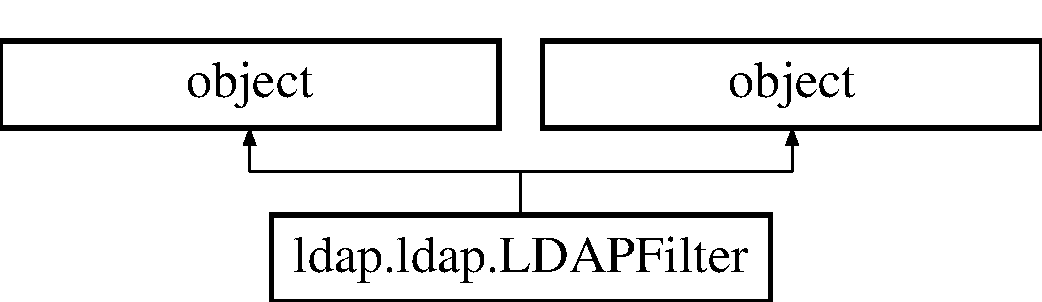
\includegraphics[height=2.000000cm]{classldap_1_1ldap_1_1LDAPFilter}
\end{center}
\end{figure}
\subsection*{Public Member Functions}
\begin{DoxyCompactItemize}
\item 
\hypertarget{classldap_1_1ldap_1_1LDAPFilter_a532a264a042d9a31f0a6752e6370c25a}{def {\bfseries \-\_\-\-\_\-init\-\_\-\-\_\-}}\label{classldap_1_1ldap_1_1LDAPFilter_a532a264a042d9a31f0a6752e6370c25a}

\item 
\hypertarget{classldap_1_1ldap_1_1LDAPFilter_a745849b29bb563fc12737948255f9151}{def {\bfseries add}}\label{classldap_1_1ldap_1_1LDAPFilter_a745849b29bb563fc12737948255f9151}

\item 
\hypertarget{classldap_1_1ldap_1_1LDAPFilter_a8001419530415812ae6f3bc2f3d87ad5}{def {\bfseries add\-\_\-filter}}\label{classldap_1_1ldap_1_1LDAPFilter_a8001419530415812ae6f3bc2f3d87ad5}

\item 
\hypertarget{classldap_1_1ldap_1_1LDAPFilter_a5ba26c6014c23a33892264bc6337db13}{def {\bfseries \-\_\-\-\_\-str\-\_\-\-\_\-}}\label{classldap_1_1ldap_1_1LDAPFilter_a5ba26c6014c23a33892264bc6337db13}

\item 
\hypertarget{classldap_1_1ldap_1_1LDAPFilter_a532a264a042d9a31f0a6752e6370c25a}{def {\bfseries \-\_\-\-\_\-init\-\_\-\-\_\-}}\label{classldap_1_1ldap_1_1LDAPFilter_a532a264a042d9a31f0a6752e6370c25a}

\item 
\hypertarget{classldap_1_1ldap_1_1LDAPFilter_a745849b29bb563fc12737948255f9151}{def {\bfseries add}}\label{classldap_1_1ldap_1_1LDAPFilter_a745849b29bb563fc12737948255f9151}

\item 
\hypertarget{classldap_1_1ldap_1_1LDAPFilter_a8001419530415812ae6f3bc2f3d87ad5}{def {\bfseries add\-\_\-filter}}\label{classldap_1_1ldap_1_1LDAPFilter_a8001419530415812ae6f3bc2f3d87ad5}

\item 
\hypertarget{classldap_1_1ldap_1_1LDAPFilter_a5ba26c6014c23a33892264bc6337db13}{def {\bfseries \-\_\-\-\_\-str\-\_\-\-\_\-}}\label{classldap_1_1ldap_1_1LDAPFilter_a5ba26c6014c23a33892264bc6337db13}

\end{DoxyCompactItemize}
\subsection*{Public Attributes}
\begin{DoxyCompactItemize}
\item 
\hypertarget{classldap_1_1ldap_1_1LDAPFilter_ad45678b172319ab01933a92f6ce44f3c}{{\bfseries filters}}\label{classldap_1_1ldap_1_1LDAPFilter_ad45678b172319ab01933a92f6ce44f3c}

\end{DoxyCompactItemize}


The documentation for this class was generated from the following files\-:\begin{DoxyCompactItemize}
\item 
/home/war/git/bmb/ldap\-\_\-pwchange/ldap/ldap.\-py\item 
/home/war/git/bmb/ldap\-\_\-pwchange/package/pk/ldap/ldap.\-py\end{DoxyCompactItemize}

\hypertarget{classldap_1_1ldap_1_1LDAPFilterItem}{\section{ldap.\-ldap.\-L\-D\-A\-P\-Filter\-Item Class Reference}
\label{classldap_1_1ldap_1_1LDAPFilterItem}\index{ldap.\-ldap.\-L\-D\-A\-P\-Filter\-Item@{ldap.\-ldap.\-L\-D\-A\-P\-Filter\-Item}}
}
Inheritance diagram for ldap.\-ldap.\-L\-D\-A\-P\-Filter\-Item\-:\begin{figure}[H]
\begin{center}
\leavevmode
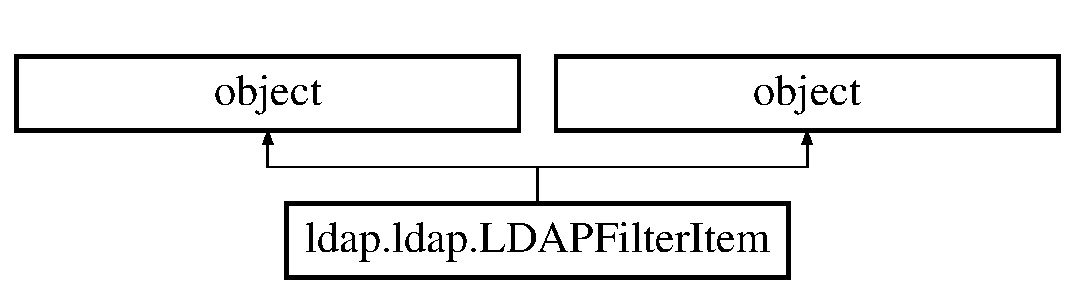
\includegraphics[height=2.000000cm]{classldap_1_1ldap_1_1LDAPFilterItem}
\end{center}
\end{figure}
\subsection*{Public Member Functions}
\begin{DoxyCompactItemize}
\item 
\hypertarget{classldap_1_1ldap_1_1LDAPFilterItem_a687ad0aea738fa8c7d05085b97ab8d3e}{def {\bfseries \-\_\-\-\_\-init\-\_\-\-\_\-}}\label{classldap_1_1ldap_1_1LDAPFilterItem_a687ad0aea738fa8c7d05085b97ab8d3e}

\item 
\hypertarget{classldap_1_1ldap_1_1LDAPFilterItem_a75d2cdee5c84d932992e69bbae14a1eb}{def {\bfseries \-\_\-\-\_\-str\-\_\-\-\_\-}}\label{classldap_1_1ldap_1_1LDAPFilterItem_a75d2cdee5c84d932992e69bbae14a1eb}

\item 
\hypertarget{classldap_1_1ldap_1_1LDAPFilterItem_a687ad0aea738fa8c7d05085b97ab8d3e}{def {\bfseries \-\_\-\-\_\-init\-\_\-\-\_\-}}\label{classldap_1_1ldap_1_1LDAPFilterItem_a687ad0aea738fa8c7d05085b97ab8d3e}

\item 
\hypertarget{classldap_1_1ldap_1_1LDAPFilterItem_a75d2cdee5c84d932992e69bbae14a1eb}{def {\bfseries \-\_\-\-\_\-str\-\_\-\-\_\-}}\label{classldap_1_1ldap_1_1LDAPFilterItem_a75d2cdee5c84d932992e69bbae14a1eb}

\end{DoxyCompactItemize}
\subsection*{Public Attributes}
\begin{DoxyCompactItemize}
\item 
\hypertarget{classldap_1_1ldap_1_1LDAPFilterItem_a0c3b5368680ad976066389008389df65}{{\bfseries attrib}}\label{classldap_1_1ldap_1_1LDAPFilterItem_a0c3b5368680ad976066389008389df65}

\item 
\hypertarget{classldap_1_1ldap_1_1LDAPFilterItem_a19832ead54944cf6a7a091991d797ec5}{{\bfseries value}}\label{classldap_1_1ldap_1_1LDAPFilterItem_a19832ead54944cf6a7a091991d797ec5}

\end{DoxyCompactItemize}


The documentation for this class was generated from the following files\-:\begin{DoxyCompactItemize}
\item 
/home/war/git/bmb/ldap\-\_\-pwchange/ldap/ldap.\-py\item 
/home/war/git/bmb/ldap\-\_\-pwchange/package/pk/ldap/ldap.\-py\end{DoxyCompactItemize}

\hypertarget{classldap_1_1ldap_1_1LDAPUserSearchFoundNoUserException}{\section{ldap.\-ldap.\-L\-D\-A\-P\-User\-Search\-Found\-No\-User\-Exception Class Reference}
\label{classldap_1_1ldap_1_1LDAPUserSearchFoundNoUserException}\index{ldap.\-ldap.\-L\-D\-A\-P\-User\-Search\-Found\-No\-User\-Exception@{ldap.\-ldap.\-L\-D\-A\-P\-User\-Search\-Found\-No\-User\-Exception}}
}
Inheritance diagram for ldap.\-ldap.\-L\-D\-A\-P\-User\-Search\-Found\-No\-User\-Exception\-:\begin{figure}[H]
\begin{center}
\leavevmode
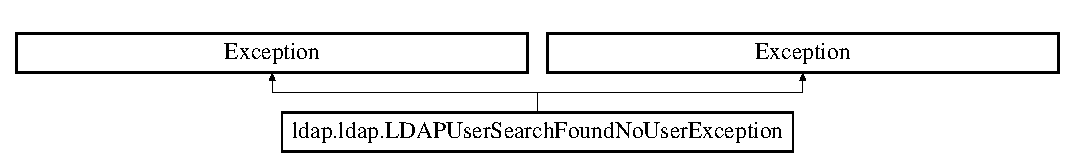
\includegraphics[height=1.812298cm]{classldap_1_1ldap_1_1LDAPUserSearchFoundNoUserException}
\end{center}
\end{figure}


The documentation for this class was generated from the following file\-:\begin{DoxyCompactItemize}
\item 
/home/war/git/bmb/ldap\-\_\-pwchange/ldap/ldap.\-py\end{DoxyCompactItemize}

\hypertarget{classldap_1_1ldap_1_1LDAPUserSearchFoundTooManyUsersException}{\section{ldap.\-ldap.\-L\-D\-A\-P\-User\-Search\-Found\-Too\-Many\-Users\-Exception Class Reference}
\label{classldap_1_1ldap_1_1LDAPUserSearchFoundTooManyUsersException}\index{ldap.\-ldap.\-L\-D\-A\-P\-User\-Search\-Found\-Too\-Many\-Users\-Exception@{ldap.\-ldap.\-L\-D\-A\-P\-User\-Search\-Found\-Too\-Many\-Users\-Exception}}
}
Inheritance diagram for ldap.\-ldap.\-L\-D\-A\-P\-User\-Search\-Found\-Too\-Many\-Users\-Exception\-:\begin{figure}[H]
\begin{center}
\leavevmode
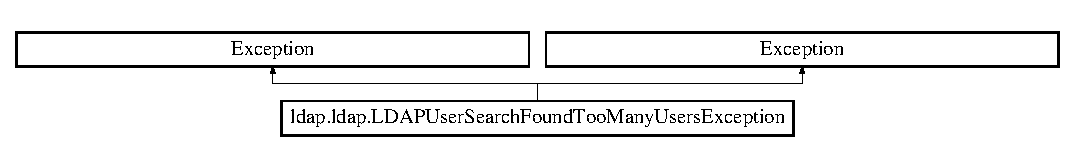
\includegraphics[height=1.590909cm]{classldap_1_1ldap_1_1LDAPUserSearchFoundTooManyUsersException}
\end{center}
\end{figure}


The documentation for this class was generated from the following file\-:\begin{DoxyCompactItemize}
\item 
/home/war/git/bmb/ldap\-\_\-pwchange/ldap/ldap.\-py\end{DoxyCompactItemize}

\hypertarget{classtools_1_1tools_1_1Log}{\section{tools.\-tools.\-Log Class Reference}
\label{classtools_1_1tools_1_1Log}\index{tools.\-tools.\-Log@{tools.\-tools.\-Log}}
}
Inheritance diagram for tools.\-tools.\-Log\-:\begin{figure}[H]
\begin{center}
\leavevmode
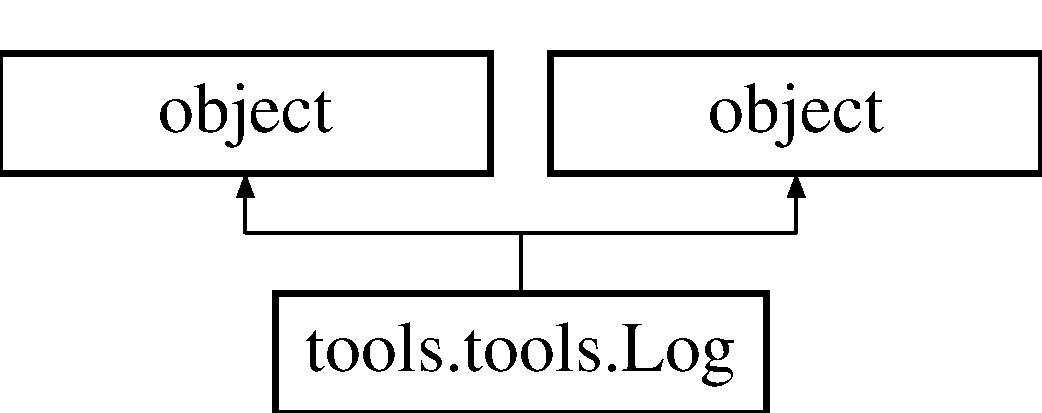
\includegraphics[height=2.000000cm]{classtools_1_1tools_1_1Log}
\end{center}
\end{figure}
\subsection*{Public Member Functions}
\begin{DoxyCompactItemize}
\item 
\hypertarget{classtools_1_1tools_1_1Log_aa3e3c9747b57d6d63cf96bc03e9cb9e3}{def {\bfseries info}}\label{classtools_1_1tools_1_1Log_aa3e3c9747b57d6d63cf96bc03e9cb9e3}

\item 
\hypertarget{classtools_1_1tools_1_1Log_a4ae4854363b96eb14b7827cb2fac1c84}{def {\bfseries error}}\label{classtools_1_1tools_1_1Log_a4ae4854363b96eb14b7827cb2fac1c84}

\item 
\hypertarget{classtools_1_1tools_1_1Log_ae7972688c982cd7f4727084e5856912b}{def {\bfseries logline}}\label{classtools_1_1tools_1_1Log_ae7972688c982cd7f4727084e5856912b}

\item 
\hypertarget{classtools_1_1tools_1_1Log_aa3e3c9747b57d6d63cf96bc03e9cb9e3}{def {\bfseries info}}\label{classtools_1_1tools_1_1Log_aa3e3c9747b57d6d63cf96bc03e9cb9e3}

\item 
\hypertarget{classtools_1_1tools_1_1Log_a4ae4854363b96eb14b7827cb2fac1c84}{def {\bfseries error}}\label{classtools_1_1tools_1_1Log_a4ae4854363b96eb14b7827cb2fac1c84}

\item 
\hypertarget{classtools_1_1tools_1_1Log_ae7972688c982cd7f4727084e5856912b}{def {\bfseries logline}}\label{classtools_1_1tools_1_1Log_ae7972688c982cd7f4727084e5856912b}

\end{DoxyCompactItemize}


The documentation for this class was generated from the following files\-:\begin{DoxyCompactItemize}
\item 
/home/war/git/bmb/ldap\-\_\-pwchange/package/pk/tools/tools.\-py\item 
/home/war/git/bmb/ldap\-\_\-pwchange/tools/tools.\-py\end{DoxyCompactItemize}

\hypertarget{classpassword_1_1password_1_1Password}{\section{password.\-password.\-Password Class Reference}
\label{classpassword_1_1password_1_1Password}\index{password.\-password.\-Password@{password.\-password.\-Password}}
}
Inheritance diagram for password.\-password.\-Password\-:\begin{figure}[H]
\begin{center}
\leavevmode
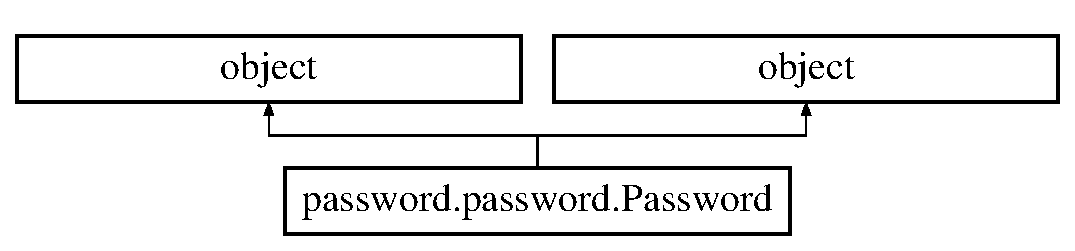
\includegraphics[height=2.000000cm]{classpassword_1_1password_1_1Password}
\end{center}
\end{figure}
\subsection*{Public Member Functions}
\begin{DoxyCompactItemize}
\item 
\hypertarget{classpassword_1_1password_1_1Password_a0a95b24e19fbdb3c2e9f12a2895ad5bd}{def {\bfseries \-\_\-\-\_\-init\-\_\-\-\_\-}}\label{classpassword_1_1password_1_1Password_a0a95b24e19fbdb3c2e9f12a2895ad5bd}

\item 
\hypertarget{classpassword_1_1password_1_1Password_ae82245d2820e1e83b5f13992f92d74ed}{def {\bfseries set\-\_\-password}}\label{classpassword_1_1password_1_1Password_ae82245d2820e1e83b5f13992f92d74ed}

\item 
\hypertarget{classpassword_1_1password_1_1Password_adf76b94e834adb438fed7eb1437579be}{def {\bfseries pw\-\_\-check}}\label{classpassword_1_1password_1_1Password_adf76b94e834adb438fed7eb1437579be}

\item 
\hypertarget{classpassword_1_1password_1_1Password_a96903b99a6210bace82f2c2a122a053f}{def {\bfseries \-\_\-\-\_\-str\-\_\-\-\_\-}}\label{classpassword_1_1password_1_1Password_a96903b99a6210bace82f2c2a122a053f}

\item 
\hypertarget{classpassword_1_1password_1_1Password_a0a95b24e19fbdb3c2e9f12a2895ad5bd}{def {\bfseries \-\_\-\-\_\-init\-\_\-\-\_\-}}\label{classpassword_1_1password_1_1Password_a0a95b24e19fbdb3c2e9f12a2895ad5bd}

\item 
\hypertarget{classpassword_1_1password_1_1Password_ae82245d2820e1e83b5f13992f92d74ed}{def {\bfseries set\-\_\-password}}\label{classpassword_1_1password_1_1Password_ae82245d2820e1e83b5f13992f92d74ed}

\item 
\hypertarget{classpassword_1_1password_1_1Password_adf76b94e834adb438fed7eb1437579be}{def {\bfseries pw\-\_\-check}}\label{classpassword_1_1password_1_1Password_adf76b94e834adb438fed7eb1437579be}

\item 
\hypertarget{classpassword_1_1password_1_1Password_a96903b99a6210bace82f2c2a122a053f}{def {\bfseries \-\_\-\-\_\-str\-\_\-\-\_\-}}\label{classpassword_1_1password_1_1Password_a96903b99a6210bace82f2c2a122a053f}

\end{DoxyCompactItemize}
\subsection*{Public Attributes}
\begin{DoxyCompactItemize}
\item 
\hypertarget{classpassword_1_1password_1_1Password_af18948ec9e5c61653ced91ce2555d9f9}{{\bfseries password}}\label{classpassword_1_1password_1_1Password_af18948ec9e5c61653ced91ce2555d9f9}

\end{DoxyCompactItemize}
\subsection*{Static Public Attributes}
\begin{DoxyCompactItemize}
\item 
\hypertarget{classpassword_1_1password_1_1Password_a09e72c280f4675f10b9202cf30b56fce}{int {\bfseries M\-I\-N\-\_\-\-P\-A\-S\-S\-W\-O\-R\-D\-\_\-\-L\-E\-N\-G\-T\-H} = 8}\label{classpassword_1_1password_1_1Password_a09e72c280f4675f10b9202cf30b56fce}

\end{DoxyCompactItemize}


The documentation for this class was generated from the following files\-:\begin{DoxyCompactItemize}
\item 
/home/war/git/bmb/ldap\-\_\-pwchange/package/pk/password/password.\-py\item 
/home/war/git/bmb/ldap\-\_\-pwchange/password/password.\-py\end{DoxyCompactItemize}

\hypertarget{classpassword_1_1password_1_1PasswordTooShortException}{\section{password.\-password.\-Password\-Too\-Short\-Exception Class Reference}
\label{classpassword_1_1password_1_1PasswordTooShortException}\index{password.\-password.\-Password\-Too\-Short\-Exception@{password.\-password.\-Password\-Too\-Short\-Exception}}
}
Inheritance diagram for password.\-password.\-Password\-Too\-Short\-Exception\-:\begin{figure}[H]
\begin{center}
\leavevmode
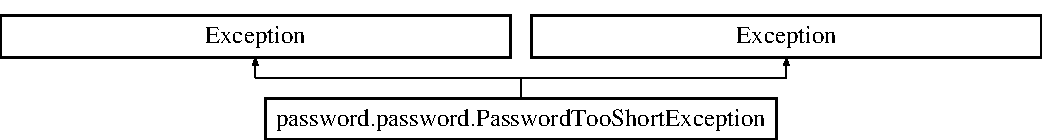
\includegraphics[height=1.885522cm]{classpassword_1_1password_1_1PasswordTooShortException}
\end{center}
\end{figure}


The documentation for this class was generated from the following file\-:\begin{DoxyCompactItemize}
\item 
/home/war/git/bmb/ldap\-\_\-pwchange/package/pk/password/password.\-py\end{DoxyCompactItemize}

\hypertarget{classservice_1_1PwChangeServer}{\section{service.\-Pw\-Change\-Server Class Reference}
\label{classservice_1_1PwChangeServer}\index{service.\-Pw\-Change\-Server@{service.\-Pw\-Change\-Server}}
}
Inheritance diagram for service.\-Pw\-Change\-Server\-:\begin{figure}[H]
\begin{center}
\leavevmode
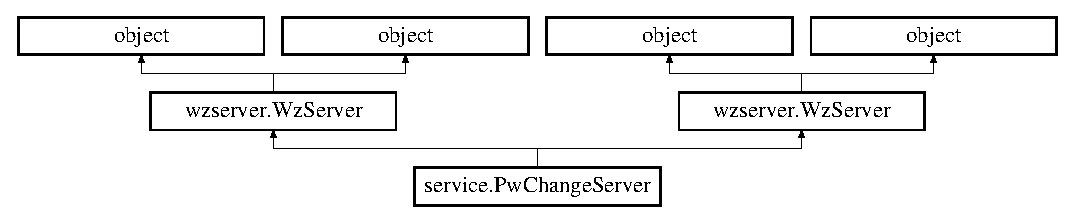
\includegraphics[height=2.530120cm]{classservice_1_1PwChangeServer}
\end{center}
\end{figure}
\subsection*{Public Member Functions}
\begin{DoxyCompactItemize}
\item 
\hypertarget{classservice_1_1PwChangeServer_a4fb6862da925977587bd74bd261a8701}{def {\bfseries \-\_\-\-\_\-init\-\_\-\-\_\-}}\label{classservice_1_1PwChangeServer_a4fb6862da925977587bd74bd261a8701}

\item 
\hypertarget{classservice_1_1PwChangeServer_a6d3a67a350bc6f6310632b93d3b9dc76}{def {\bfseries on\-\_\-change}}\label{classservice_1_1PwChangeServer_a6d3a67a350bc6f6310632b93d3b9dc76}

\item 
\hypertarget{classservice_1_1PwChangeServer_a1364ecbaf8211611b793345d73249eac}{def {\bfseries on\-\_\-final}}\label{classservice_1_1PwChangeServer_a1364ecbaf8211611b793345d73249eac}

\item 
\hypertarget{classservice_1_1PwChangeServer_a4fb6862da925977587bd74bd261a8701}{def {\bfseries \-\_\-\-\_\-init\-\_\-\-\_\-}}\label{classservice_1_1PwChangeServer_a4fb6862da925977587bd74bd261a8701}

\item 
\hypertarget{classservice_1_1PwChangeServer_a6d3a67a350bc6f6310632b93d3b9dc76}{def {\bfseries on\-\_\-change}}\label{classservice_1_1PwChangeServer_a6d3a67a350bc6f6310632b93d3b9dc76}

\item 
\hypertarget{classservice_1_1PwChangeServer_a1364ecbaf8211611b793345d73249eac}{def {\bfseries on\-\_\-final}}\label{classservice_1_1PwChangeServer_a1364ecbaf8211611b793345d73249eac}

\end{DoxyCompactItemize}
\subsection*{Public Attributes}
\begin{DoxyCompactItemize}
\item 
\hypertarget{classservice_1_1PwChangeServer_a79c4db6ac155df4b35e5c9c93fe3ce2c}{{\bfseries url\-\_\-map}}\label{classservice_1_1PwChangeServer_a79c4db6ac155df4b35e5c9c93fe3ce2c}

\item 
\hypertarget{classservice_1_1PwChangeServer_ad9074b7e33eeb288ad9696f7acd657fd}{{\bfseries ldap}}\label{classservice_1_1PwChangeServer_ad9074b7e33eeb288ad9696f7acd657fd}

\end{DoxyCompactItemize}


The documentation for this class was generated from the following files\-:\begin{DoxyCompactItemize}
\item 
/home/war/git/bmb/ldap\-\_\-pwchange/package/pk/service.\-py\item 
/home/war/git/bmb/ldap\-\_\-pwchange/service.\-py\end{DoxyCompactItemize}

\hypertarget{classsession_1_1SessionStore}{\section{session.\-Session\-Store Class Reference}
\label{classsession_1_1SessionStore}\index{session.\-Session\-Store@{session.\-Session\-Store}}
}
Inheritance diagram for session.\-Session\-Store\-:\begin{figure}[H]
\begin{center}
\leavevmode
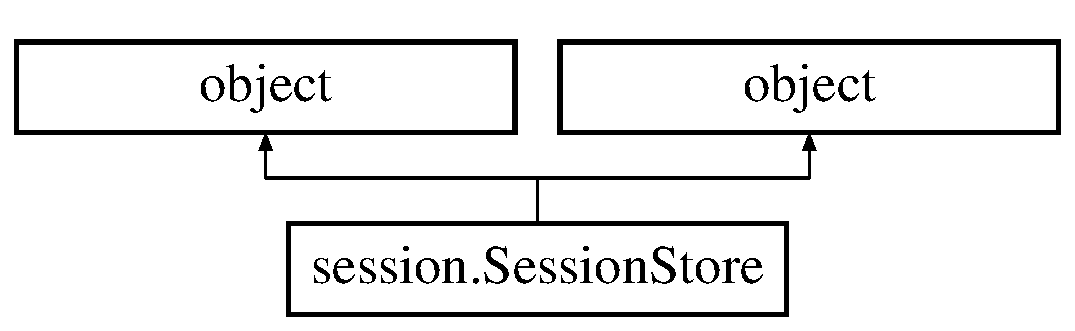
\includegraphics[height=2.000000cm]{classsession_1_1SessionStore}
\end{center}
\end{figure}
\subsection*{Public Member Functions}
\begin{DoxyCompactItemize}
\item 
\hypertarget{classsession_1_1SessionStore_aa8a9de02e72668c7870695ecb96486cc}{def {\bfseries new}}\label{classsession_1_1SessionStore_aa8a9de02e72668c7870695ecb96486cc}

\item 
\hypertarget{classsession_1_1SessionStore_a99853f3f868737b2dbc2928747cd9c7a}{def {\bfseries get}}\label{classsession_1_1SessionStore_a99853f3f868737b2dbc2928747cd9c7a}

\item 
\hypertarget{classsession_1_1SessionStore_a4add87957b4e0c37501693d2e5a095bc}{def {\bfseries get\-\_\-or\-\_\-new}}\label{classsession_1_1SessionStore_a4add87957b4e0c37501693d2e5a095bc}

\item 
\hypertarget{classsession_1_1SessionStore_a46e93026fe273ce3b050e0f1b88d05b3}{def {\bfseries save}}\label{classsession_1_1SessionStore_a46e93026fe273ce3b050e0f1b88d05b3}

\item 
\hypertarget{classsession_1_1SessionStore_aa8a9de02e72668c7870695ecb96486cc}{def {\bfseries new}}\label{classsession_1_1SessionStore_aa8a9de02e72668c7870695ecb96486cc}

\item 
\hypertarget{classsession_1_1SessionStore_a99853f3f868737b2dbc2928747cd9c7a}{def {\bfseries get}}\label{classsession_1_1SessionStore_a99853f3f868737b2dbc2928747cd9c7a}

\item 
\hypertarget{classsession_1_1SessionStore_a4add87957b4e0c37501693d2e5a095bc}{def {\bfseries get\-\_\-or\-\_\-new}}\label{classsession_1_1SessionStore_a4add87957b4e0c37501693d2e5a095bc}

\item 
\hypertarget{classsession_1_1SessionStore_a46e93026fe273ce3b050e0f1b88d05b3}{def {\bfseries save}}\label{classsession_1_1SessionStore_a46e93026fe273ce3b050e0f1b88d05b3}

\end{DoxyCompactItemize}
\subsection*{Static Public Attributes}
\begin{DoxyCompactItemize}
\item 
\hypertarget{classsession_1_1SessionStore_a8593aee7fce30397f65ce73af095bc12}{tuple {\bfseries path} = tempfile.\-gettempdir()}\label{classsession_1_1SessionStore_a8593aee7fce30397f65ce73af095bc12}

\item 
\hypertarget{classsession_1_1SessionStore_a066f616244e637822f9687d3e067c715}{tuple {\bfseries session\-\_\-store} = Filesystem\-Session\-Store(path)}\label{classsession_1_1SessionStore_a066f616244e637822f9687d3e067c715}

\end{DoxyCompactItemize}


The documentation for this class was generated from the following files\-:\begin{DoxyCompactItemize}
\item 
/home/war/git/bmb/ldap\-\_\-pwchange/package/pk/session.\-py\item 
/home/war/git/bmb/ldap\-\_\-pwchange/session.\-py\end{DoxyCompactItemize}

\hypertarget{classwzserver_1_1WzServer}{\section{wzserver.\-Wz\-Server Class Reference}
\label{classwzserver_1_1WzServer}\index{wzserver.\-Wz\-Server@{wzserver.\-Wz\-Server}}
}
Inheritance diagram for wzserver.\-Wz\-Server\-:\begin{figure}[H]
\begin{center}
\leavevmode
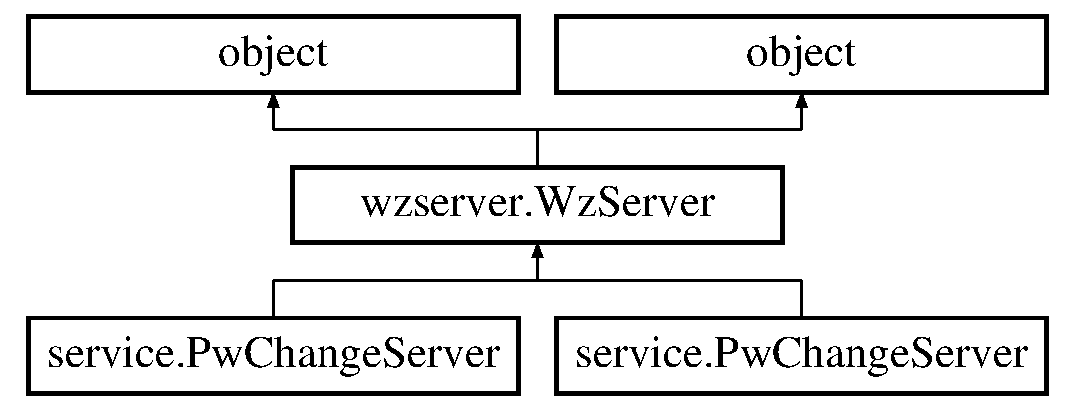
\includegraphics[height=3.000000cm]{classwzserver_1_1WzServer}
\end{center}
\end{figure}
\subsection*{Public Member Functions}
\begin{DoxyCompactItemize}
\item 
\hypertarget{classwzserver_1_1WzServer_a3650c7152ba300dd9dd6cde4927406df}{def {\bfseries \-\_\-\-\_\-init\-\_\-\-\_\-}}\label{classwzserver_1_1WzServer_a3650c7152ba300dd9dd6cde4927406df}

\item 
\hypertarget{classwzserver_1_1WzServer_a13661c6372da0e23dc61ec61e3187d3a}{def {\bfseries render\-\_\-template}}\label{classwzserver_1_1WzServer_a13661c6372da0e23dc61ec61e3187d3a}

\item 
\hypertarget{classwzserver_1_1WzServer_a42cd1fa0c1034bfc435c63d2dadf1494}{def {\bfseries dispatch\-\_\-request}}\label{classwzserver_1_1WzServer_a42cd1fa0c1034bfc435c63d2dadf1494}

\item 
\hypertarget{classwzserver_1_1WzServer_ad9ace307e3936d8ae3d2b42c23208e8b}{def {\bfseries wsgi\-\_\-app}}\label{classwzserver_1_1WzServer_ad9ace307e3936d8ae3d2b42c23208e8b}

\item 
\hypertarget{classwzserver_1_1WzServer_a7becba76cff1dd16f084d613c9ce2238}{def {\bfseries \-\_\-\-\_\-call\-\_\-\-\_\-}}\label{classwzserver_1_1WzServer_a7becba76cff1dd16f084d613c9ce2238}

\item 
\hypertarget{classwzserver_1_1WzServer_adda0194ac2db4cae016add3d6bebf1be}{def {\bfseries save\-\_\-session\-\_\-data}}\label{classwzserver_1_1WzServer_adda0194ac2db4cae016add3d6bebf1be}

\item 
\hypertarget{classwzserver_1_1WzServer_a3650c7152ba300dd9dd6cde4927406df}{def {\bfseries \-\_\-\-\_\-init\-\_\-\-\_\-}}\label{classwzserver_1_1WzServer_a3650c7152ba300dd9dd6cde4927406df}

\item 
\hypertarget{classwzserver_1_1WzServer_a13661c6372da0e23dc61ec61e3187d3a}{def {\bfseries render\-\_\-template}}\label{classwzserver_1_1WzServer_a13661c6372da0e23dc61ec61e3187d3a}

\item 
\hypertarget{classwzserver_1_1WzServer_a42cd1fa0c1034bfc435c63d2dadf1494}{def {\bfseries dispatch\-\_\-request}}\label{classwzserver_1_1WzServer_a42cd1fa0c1034bfc435c63d2dadf1494}

\item 
\hypertarget{classwzserver_1_1WzServer_ad9ace307e3936d8ae3d2b42c23208e8b}{def {\bfseries wsgi\-\_\-app}}\label{classwzserver_1_1WzServer_ad9ace307e3936d8ae3d2b42c23208e8b}

\item 
\hypertarget{classwzserver_1_1WzServer_a7becba76cff1dd16f084d613c9ce2238}{def {\bfseries \-\_\-\-\_\-call\-\_\-\-\_\-}}\label{classwzserver_1_1WzServer_a7becba76cff1dd16f084d613c9ce2238}

\item 
\hypertarget{classwzserver_1_1WzServer_adda0194ac2db4cae016add3d6bebf1be}{def {\bfseries save\-\_\-session\-\_\-data}}\label{classwzserver_1_1WzServer_adda0194ac2db4cae016add3d6bebf1be}

\end{DoxyCompactItemize}
\subsection*{Public Attributes}
\begin{DoxyCompactItemize}
\item 
\hypertarget{classwzserver_1_1WzServer_a7272469b9646f4e9e36848bd985864a9}{{\bfseries session\-\_\-store}}\label{classwzserver_1_1WzServer_a7272469b9646f4e9e36848bd985864a9}

\item 
\hypertarget{classwzserver_1_1WzServer_a09ef23bbd3f0c78456302e61fc0a3d48}{{\bfseries jinja\-\_\-env}}\label{classwzserver_1_1WzServer_a09ef23bbd3f0c78456302e61fc0a3d48}

\item 
\hypertarget{classwzserver_1_1WzServer_ae2c3b8ed8efdae92a62fd755a48df995}{{\bfseries url\-\_\-map}}\label{classwzserver_1_1WzServer_ae2c3b8ed8efdae92a62fd755a48df995}

\end{DoxyCompactItemize}


The documentation for this class was generated from the following files\-:\begin{DoxyCompactItemize}
\item 
/home/war/git/bmb/ldap\-\_\-pwchange/package/pk/wzserver.\-py\item 
/home/war/git/bmb/ldap\-\_\-pwchange/wzserver.\-py\end{DoxyCompactItemize}

%--- End generated contents ---

% Index
\newpage
\phantomsection
\addcontentsline{toc}{part}{Index}
\printindex

\end{document}
